\documentclass{beamer}


\usetheme{AnnArbor}
\usecolortheme{default}


\title{Models of Complex Adaptive Social Systems}
%\subtitle{Complex Systems Engineering}
\author{Steve Mazza}
\institute[Naval Postgraduate School]
{ 
    Naval Postgraduate School \\
    Monterey, CA \\
    
\includegraphics[height=3cm]{images/NPS_logo.jpg}
}
\date {SE4940, Spring/2014}
\subject{Complex Systems Engineering}


\begin{document}

\frame{\titlepage}


\frame{{A Basic Framework}
  The elements of the eightfold path can be mapped to key modeling issues in complex social systems.
}

\frame{{The Eightfold Way}
  \begin{columns}[c]
    \column{0.4\textwidth}
      \begin{itemize}
        \item Wisdom
          \begin{itemize}
            \item Right View
            \item Right Intention
          \end{itemize}
        \item Ethical Conduct
          \begin{itemize}
            \item Right Speech
            \item Right Action
            \item Right Livelihood
          \end{itemize}
        \item Concentration
          \begin{itemize}
            \item Right Effort
            \item Right Mindfulness
            \item Right Concentration
          \end{itemize}
      \end{itemize}
    \column{0.6\textwidth}
    \begin{center}
      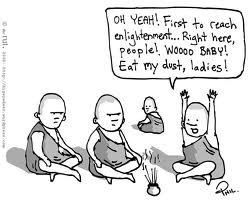
\includegraphics[scale=0.75]{images/noblecomix.jpg}
    \end{center}
  \end{columns}
}

\frame{{The Eightfold Way}
  \framesubtitle{Right View}
  \begin{itemize}
    \item Information the agent sees.
    \item Often no too much information competes for attention.
    \item Information is often processed through the lens of previous experience (internal information).
    \item Information may come from another agent with (or without) bias.
    \item Timing of information and how it flows can be very important.
  \end{itemize}
}

\frame{{The Eightfold Way}
  \framesubtitle{Right Intention}
  \begin{itemize}
    \item Goals of the agent.
    \item May be explicit or implicit.
    \item Place strong forces on model's behavior.
    \item Often most interesting when the intentions are at odds with the model's outcome.
  \end{itemize}
}

\frame{{The Eightfold Way}
  \framesubtitle{Right Speech}
  \begin{itemize}
    \item Information agents send to others.
    \item May be action or more explicit.
    \item Varies by type based on model parameters.
    \item An important part of many complex adaptive social systems.
  \end{itemize}
}

\frame{{The Eightfold Way}
  \framesubtitle{Right Action}
  \begin{itemize}
    \item All the interactions that occur among the agents.
    \item Depend on \emph{space,} which can be physical or logical (e.g., friendships).
    \item May be externally coordinated.
    \item Can by synchronous or asynchronous.
    \item Type of updating can have a large impact on the outcome of the model.
  \end{itemize}
}

\frame{{The Eightfold Way}
  \framesubtitle{Right Livelihood}
  \begin{itemize}
    \item Payoffs that accrue to the agents.
    \item Payoffs result in benefits or costs.
    \item Payoffs often drive adaptation (e.g., agents reproduce based on their performance).
    \item Payoffs can drive activation order, giving preference to higher performing agents.
  \end{itemize}
}

\frame{{The Eightfold Way}
  \framesubtitle{Right Effort}
  \begin{itemize}
    \item Includes agents' strategies and actions.
    \item These may be guided by extreme thought and care or by intuitions, emotions, and gut instincts.
    \item Rules adopted by agents to govern behavior may be fixed or adaptive.
    \item Rules may appear to be simple or complex.
  \end{itemize}
}

\frame{{The Eightfold Way}
  \framesubtitle{Right Mindfulness}
  \begin{itemize}
    \item The level of cognition employed by the agent.
    \item Mindfulness differs between social and physical agents (e.g., people vs.\ subatomic particles).
    \item Social agents may employ mental models that inform their behavior.
    \item May be an under-explored factor in some types of models (e.g., economic).
  \end{itemize}
}

\frame{{The Eightfold Way}
  \framesubtitle{Right Concentration}
  \begin{itemize}
    \item The focus of the model; it must be just sufficient to capture the phenomenon of interest.
    \item Agent diversity enriches the model.
    \item Diversity can be behavioral or historical or may rely on differential access to information or underlying characteristics. 
  \end{itemize}
}

\frame{{Smoke and Mirrors: the Forest Fire Model}
  \framesubtitle{A Simple Model}
  We begin with the simplest model of forest fires.
  \begin{itemize}
    \item 1-dimensional model
    \item Fixed, homogeneous rules.
    \item At one time step trees grow with probability $g$.
    \item At the other time step trees burn with probability $f$, taking out all adjacent trees.
    \item The cycle repeats.
  \end{itemize}
  Optimizing for production favors a growth rate of 43\% at which point density becomes a compelling factor as fire breaks become too few.
}

\frame{{Smoke and Mirrors: the Forest Fire Model}
  \framesubtitle{Homogeneous Adaptation}
  \begin{block}{Rule:}
    Forests with higher productivity survive.  Those with lower productivity are killed off and replaced by new ones with random growth rates.
  \end{block}
  By varying the model rules and allowing rule-set selection based on survival (fitness), we expect to see the forest growth rate approach the critical value, $g$.
}

\frame{{Smoke and Mirrors: the Forest Fire Model}
  \framesubtitle{Heterogeneous Adaptation}
  \begin{block}{Rule:}
    If a tree on a site would have burned down, then decrease the growth rate; otherwise, increase it.
  \end{block}
  Applying a varying rule-set with finer granularity (i.e., to individual trees) results in adaptation that is individually decided but which suits the collective good.  Over enough time this results in substantially growth rate.
}

\frame{{Smoke and Mirrors: the Forest Fire Model}
  \framesubtitle{Adding More Intelligence}
  \begin{block}{Rule:}
    Individual agents construct independent models of the system, making assumptions about their neighbors behavior which drives their own.
  \end{block}
  This strategy is far more sophisticated than previous models and leads to some potentially complex behavioral dynamics, but not necessarily any better solution.
}

\frame{{Smoke and Mirrors: the Forest Fire Model}
  \framesubtitle{Omnicient Closure}
  Allowing for altruistic behavior, it is possible (albeit difficult and unlikely) to achieve an optimal and stable state.

  This model is still not likely to out-perform heterogeneous adaptation, which converges steadily on an optimal solution and provides considerable stability.
}

\frame{{Smoke and Mirrors: the Forest Fire Model}
  \framesubtitle{Banks}
  By applying different labels, the same models can be applied to bank failures and urban migration, among other problems.
}

\frame{{Eight Folding into One}
  Ultimately, none of the models presented falls into the category of Universal Computer.  The author reminds us of Turing's findings regarding the Halting Problem: that general propositions about universal computers are undecidable.

  Notwithstanding, this does not diminish the value of having applied a model toward achieving a solution to a particular problem.
}

\frame{{Conclusion}
  \begin{itemize}
    \item Different levels of adaptation impact behavior.  The emergence of firewalls in the forest fire model demonstrates how collective intelligence can arise.  Miller points to the interesting space between fixed rules and cognitive closure, referring to it as, ``both clever and messy.''
    \item Applying different labels allow us to use the same model in a variety of different domains across the same problem class (e.g., forest fires, bank failures, urban-suburban migration).
    \item ``The promise of uncovering deep connections among apparently disparate complex social systems is an important one.''
  \end{itemize}
}

\frame{{Complex Adaptive Social Systems in One Dimension}
  \begin{block}{Goal}
    We want to have simple models that reveal something basic about complex adaptive social systems.
  \end{block}
  Modeling is an iterative process by which we arrive at a better understanding of complex systems.
  \begin{itemize}
    \item Begin with simple assumptions and see where they lead.
    \item Use these results to create better models which lead to more exact results.
  \end{itemize}
}

\frame{{Cellular Automata}
  Simple homogeneous rules can result in surprising behavior.  Moments of coherence are mixed with \emph{perpetual novelty.}

  Wolfram categorized rules into four classes (previously discussed at length).  These rules allow us to make predictions about behavior based on structure and initial conditions.
} 

\frame{{Social Cellular Automata}
  Modeling social systems means accepting a couple of limitations.
  \begin{enumerate}
    \item All agents operate under the same rules.
    \item History is summarily discarded (is this really different that reality).
  \end{enumerate}
  Rule sets can be dramatically reduced by imposing both observational and outcome symmetry.  Miller selects four rules that appear to be representative of broad classes of rule sets under these constraints, but lays no claim to specificity.
}

\frame{{Majority Rules}
  \begin{block}{Rule:}
    Each agent will look a distance of $k$ sites and alter its action if it is in the minority.
  \end{block} 

  Different updating rules may result in very different equilibrium outcomes.

  \begin{exampleblock}{Claim 8.3.1}
    Any $N$-Site $k$-Majority Rule model with asynchronous updating attains fixed-point equilibrium in in finite time.
  \end{exampleblock}
  Proof is contained on page 127 of Miller.

  Randomness introduces mistakes which can help avoid local maxima and minima.
}

\frame{{The Edge of Chaos}
  \begin{block}{What Is the Edge}
    ``The edge of chaos captures the essence of all interesting adaptive systems as they evolve to this boundary between stable order and unstable chaos.''
  \end{block}

The edge is in the rules, not the resulting phase space.  We use $\lambda$, which equals the percentage of all rule table entries that map to a predefined quiescent state.  Thus, as $\lambda$ approaches 1/2 (in between the two extremes, 0 and 1), chaos becomes more prevalent.
}

\frame{{Questions?}
	\begin{center}
		
\includegraphics[width=.7\textwidth]{images/fin.png}
	\end{center}
}

\end{document}
